\chapter{The quasi-local approach: trapping horizons}
\label{s:loc}

\minitoc

\section{Introduction}

This chapter is in a draft stage.

\section{Trapped surfaces and singularity theorems}

\subsection{Trapped surfaces}

The concept of trapped surfaces has been introduced in Sec.~\ref{s:neh:trapped_surfaces}
(see in particular Fig.~\ref{f:neh:trapped_surf}). Let us recall that
a submanifold $\Sp$ of a $n$-dimensional spacetime ($n\ge 3$) is
a \defin{trapped surface}\index{trapped!surface} iff (i) $\Sp$ is a compact $(n-2)$-dimensional manifold
(without boundary), (ii) $\Sp$ is spacelike (positive definite induced metric)
and the two systems of null geodesics emerging orthogonally from $\Sp$ towards the future
locally converge, i.e. they have negative expansions at $\Sp$:
$\theta_{(\wl)} < 0$ and $\theta_{(\w{k})} < 0$ [Eq.~(\ref{e:neh:def_trapped_surf})],
$\wl$ and $\w{k}$ being
future-directed vectors tangent to these geodesics.

\begin{remark}
Trapped surfaces are sometimes called
\emph{closed trapped surfaces}\index{closed!trapped surface}\index{trapped!surface!closed --} (e.g. \cite{Penro65,HawkiE73}),
to stress their closed manifold aspect (compact without boundary).
We follow here the textbooks \cite{MisneTW73,Wald84} and call them merely
\emph{trapped surfaces}.
\end{remark}

\begin{example}[trapped surfaces in Schwarzschild spacetime]
Let $(\M,\w{g})$ be the Schwarzschild spacetime as defined in Sec.~\ref{s:sch:time_orientation} [Eq.~(\ref{s:sch:def_Schwarz_spacetime})]; it is entirely covered by the ingoing Eddington-Finkelstein coordinates
$(\ti,r,\th,\ph)$. Let $\Sp$ be any surface $(\ti,r) = \mathrm{const}$.
$\Sp$ is diffeomorphic to $\mathbb{S}^2$ and thus compact.
Moreover, from Eq.~(\ref{e:sch:Schwarz_metric_EF}), the metric induced by $\w{g}$
on $\Sp$ is $\w{q} = r^2 (\D\th^2 + \sin^2\th\D\ph^2)$, which is clearly positive definite, so
that $\Sp$ is spacelike. One reads also on the expression of $\w{q}$
that the area of  $\Sp$ is simply $A = 4\pi r^2$ (i.e. $r$ is the areal radius, cf. Sec.~\ref{s:sch:static_spher}).
If $\Sp$ is located in the black hole interior, i.e. if $0<r < 2m$,
Property~\ref{p:sch:r_decreasing} implies that $A$ is decreasing along any future-directed null
geodesic. It follows that $\Sp$ is trapped. On the contrary, if located in the black hole exterior
($r> 2m$), $\Sp$ is untrapped. This can be checked on Fig.~\ref{f:sch:rad_null_geod_EF},
where it appears clearly that, in the region $r>2m$, $r$ is increasing along the outgoing radial null geodesics, which are normal to $\Sp$.
\end{example}

\begin{figure}
\centerline{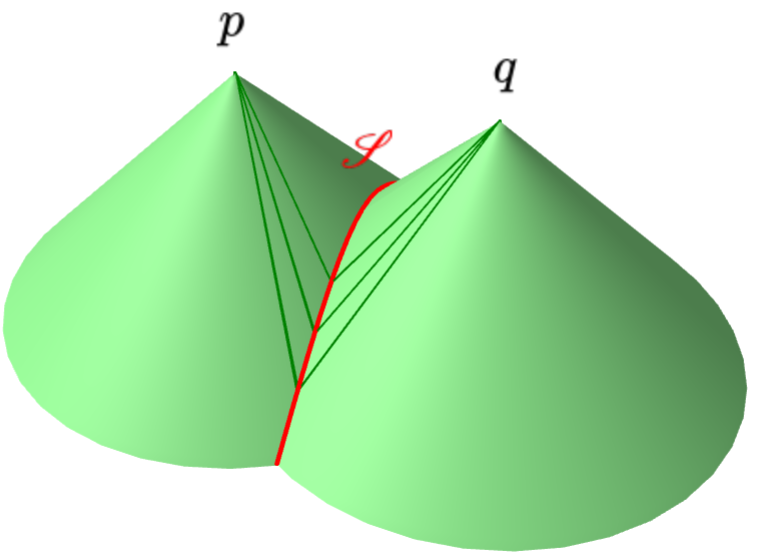
\includegraphics[width=0.6\textwidth]{loc_cone_intersect.png}}
\caption[]{\label{f:loc:cone_intersect} \footnotesize
Intersection $\Sp$ (red curve) of the past light cones of two points $p$ and $q$ in Minkowski spacetime.
Some light rays emerging from $\Sp$ in the two orthogonal null directions are depicted; the two sets
of light rays are both converging. Yet $\Sp$ is not trapped because it is not compact.
\textsl{[Figure generated by the notebook \ref{s:sam:loc_cone_intersect}]}
}
\end{figure}

The hypothesis of \emph{compact} manifold is crucial in the definition of a
trapped surface. Without it, there would exist trapped surfaces in Minkowski
spacetime, as the following example shows.

\begin{example}[a counter-example in Minkowkski spacetime]
Let us consider the intersection $\Sp$ of the past light cones $\mathscr{C}_p$ and $\mathscr{C}_q$
of two points $p$ and $q$ of Minkowski spacetime (cf. Fig.~\ref{f:loc:cone_intersect}).
Being a cross-section of the null hypersurface $\mathscr{C}_p$ (or $\mathscr{C}_q$),
$\Sp$ is a spacelike surface (Property~\ref{p:def:spacelike_cs}).
Moreover the null directions $\w{k}$ and $\wl$ normal to it are given by the null generators of
$\mathscr{C}_p$ (since $\Sp$ is a cross-section of $\mathscr{C}_p$)
and of $\mathscr{C}_q$ (since $\Sp$ is a cross-section of $\mathscr{C}_q$).
Because $\mathscr{C}_p$ and $\mathscr{C}_q$ are past light cones, one has clearly
$\theta_{(\wl)} < 0$ and $\theta_{(\w{k})} < 0$.
However, $\Sp$ fails to be a trapped surface for it is not compact. Truncating the light cones
would not help, because this would make $\Sp$ a manifold with boundary and hence not a closed one.
\end{example}


\subsection{Penrose's singularity theorem}

\begin{prop}[Penrose's singularity theorem \textnormal{(Penrose 1965 \cite{Penro65})}]
Let $(\M,\w{g})$ be a $n$-dimensional spacetime ($n\ge 3$) such that
\begin{itemize}
\item $(\M,\w{g})$ admits a non-compact Cauchy surface $\Sigma$;
\item the null energy condition (\ref{e:neh:null_energy_cond}) holds on $\M$:
for any null vector $\wl$, $\w{R}(\wl, \wl) \geq 0$, where $\w{R}$ is
$\w{g}$'s Ricci tensor;
\item there exists a trapped surface $\Sp$.
\end{itemize}
Then there exists at least one null geodesic emerging orthogonally from $\Sp$
that is incomplete towards the future.
\end{prop}

%%%%%%%%%%%%%%%%%%%%%%%%%%%%%%%%%%%%%%%%%%%%%%%%%%%%%%%%%%%%%%%%%%%%%%%%%%%%%%%

\section{Trapping horizons}


